\documentclass{beamer}
\usetheme{Madrid}

% escreve textos gerados em portugues
\usepackage[brazilian]{babel}
% aceita unicode
\usepackage[utf8]{inputenc}

\author[Andre Esteve and Zhenlei Ji]{
Andre Petris Esteve - \texttt{andreesteve@gmail.com}\\
Zhenlei Ji - \texttt{zhenlei.ji@gmail.com}}
\institute[IC\textbackslash UNICAMP]{
MC806 - Operational System Topics\\}

\title[Linux VFS]{Linux Virtual File System}
\subtitle[]{The linux VFS and FUSE - File System in User Space}

\date[10/20/2011]{October 20th, 2011}

\begin{document}

%--- create section frame for every new section --%
\AtBeginSection[]
{
   \begin{frame}
       \frametitle{Agenda}
       \tableofcontents[currentsection]
   \end{frame}
}

\begin{frame}[plain]
  \titlepage
\end{frame}

%--- content -------------------------------------%
\begin{frame}{Agenda}
  \tableofcontents
\end{frame}

\section{Objectives}

\begin{frame}{Objectives}

  \begin{block}{What do we want?}

	\begin{itemize}[<+->]

		\item{View the Linux's Virtual File System as a series of object oriented entities (classes and objects)}

		\item{Construct UML models to easy understanding}
		
		\item{Provide initial information so one can start developing a file system module for the Linux kernel}
	
	\end{itemize}

  \end{block}

\end{frame}

\begin{frame}{Warning}

  \begin{block}{Please note!}

	\begin{itemize}[<+->]

		\item{All information here is based extensively on linux kernel 3.1-rc8 source code}

		\item{Some models are represented at a certain level of abstraction and may omit some implementation information}
	
	\end{itemize}

  \end{block}

\end{frame}

\section{Linux's Virtual File System Overview}

\begin{frame}{What's Linux's Virtual File System}

  \begin{block}{Definition}

	The Virtual File System (also known as the Virtual Filesystem Switch)
	is the software layer in the kernel that provides the filesystem
	interface to userspace programs. It also provides an abstraction
	within the kernel which allows different filesystem implementations to
	coexist. \footnotemark

  \end{block}

	\footnotetext[1]{Overview of the Linux Virtual File System, Richard Gooch, from Linux "documentation"}

\end{frame}

\begin{frame}{Linux's Virtual File System Overview}

	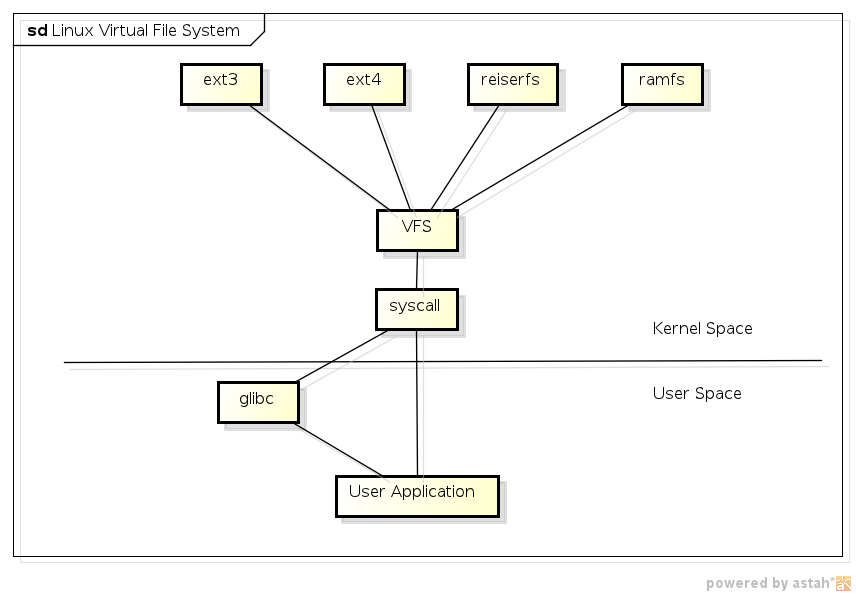
\includegraphics[scale=0.5]{img/vfs_overview.png}

\end{frame}

\begin{frame}{Linux's Virtual File System Overview}

	\begin{itemize}[<+->]
	
		\item[$\bullet$]{Abstraction layer to allow different fs\footnotemark[1] to coexist}	
		\item[$\bullet$]{Only point of access to fs calls}
		\item[$\bullet$]{Implements common fs operations}
			\begin{itemize}
				\item[$-$]{Common inicialization operations}
				\item[$-$]{Mounting (at a certain level) and managing mount points}
				\item[$-$]{Path lookup}
				\item[$-$]{Caching}
			\end{itemize}	
	\end{itemize}

	\footnotetext[1]{Short for "file system"}

\end{frame}

\begin{frame}{Linux's Virtual File System Overview}

	\begin{block}{How is a file system implemented?}
		With loadable kernel modules\footnotemark[1] (LKM), or just modules for short.
	\end{block}

	\vspace{15pt}
	
	\pause

	\begin{itemize}[<+->]
	
		\item[$\bullet$]{It's possible to compile a LKM with the base kernel}
		\item[$\bullet$]{Or just load the LKM during system usage}

	\end{itemize}

	\footnotetext[1]{For an extensive discussion about LKM, see: \texttt{http://www.tldp.org/HOWTO/Module-HOWTO/}}

\end{frame}

\section{Linux's Virtual File System Core Elements}

\begin{frame}{Linux's Virtual File System Core Elements}

	\begin{description}[<+->]\itemsep4pt
			
		\item[file\_system\_type]{Information about a specific fs type}
		\item[vfsmount]{Mount point information}		
		\item[super\_block]{Represents a mounted file system}
		\item[inode]{Information about a file (on disk, memory or network)}
		\item[dentry]{A directory entry}
		\item[file]{A file abstraction - points to a inode}

		\vspace{15pt}

		\item{Note: Every element, except vfsmount, is defined at include/linux/fs.h.}

	\end{description}

\end{frame}

\begin{frame}{Linux's Virtual File System Core Elements}
	
	\center{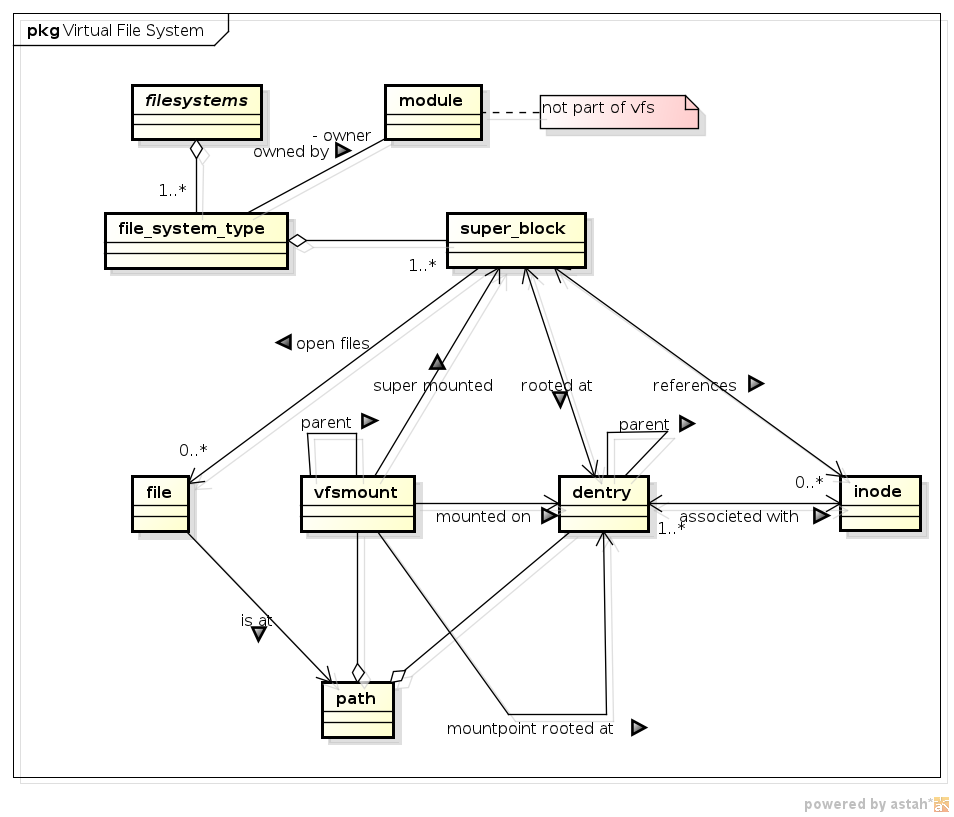
\includegraphics[scale=0.35]{img/vfs_elements_simple.png}}

\end{frame}

\subsection{file\_system\_type}

\begin{frame}{file\_system\_type}
	
	\center{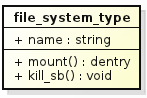
\includegraphics{img/file_system_type.png}}
	
\end{frame}

\begin{frame}{file\_system\_type}
	
	\begin{itemize}[<+->]
	
		\item[$\bullet$]{Represents a file system type (e.g. ext3, nfs, fuse)}
		\item[$\bullet$]{fs/filesystems.c has a linked list of file system types}
		\item[$\bullet$]{Each file system type must have a unique name}
		\item[$\bullet$]{Each file system type has a linked list of super blocks in use (i.e. mounted)}		
		\item[$\bullet$]{Each file system type is owned by a module (which implements it)}
		\item[$\bullet$]{Each file system type has a function to mount a (possibly new) instance of the file system}
		
	\end{itemize}

\end{frame}

\subsection{vfsmount}

\begin{frame}{vfsmount}
	
	\center{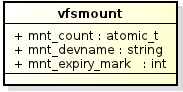
\includegraphics{img/vfsmount.png}}
	
\end{frame}

\begin{frame}{vfsmount}
	
	\begin{itemize}[<+->]

		\item[$\bullet$]{Defined at include/linux/mount.h}	

		\item[$\bullet$]{Store information about a mount point}
			\begin{itemize}
				\item[$-$]{Device name (if any)}
				\item[$-$]{Use count (if 0 the fs could be unmounted if mnt\_expiry\_mark is set) }
			\end{itemize}	
		
		\item[$\bullet$]{Refers to the parent mount point (the one its mounted on) and has a list of mounted children}
		\item[$\bullet$]{Points to the parent (mount point) dentry root}
		\item[$\bullet$]{Has a dentry for its own root}
		\item[$\bullet$]{Has the super block of the mounted file system}		
		\item[$\bullet$]{Not directly handled by a file system implementation}
		
	\end{itemize}

\end{frame}

\subsection{super\_block}

\begin{frame}{super\_block}
	
	\center{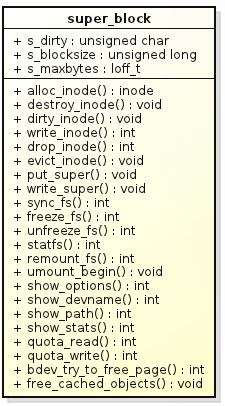
\includegraphics[scale=0.65]{img/super_block.png}}
	
\end{frame}

\begin{frame}{super\_block}
	
	\begin{itemize}[<+->]

		\item[$\bullet$]{Represents a file system instance}
		\item[$\bullet$]{When the file system is disk based, the super block usualy is persisted on disk}		
		\item[$\bullet$]{It's kept on memory, but there's a dirty flag so it can eventualy be flush to disk (for disk based fs)}
		\item[$\bullet$]{Defines file system's properties}
			\begin{itemize}
				\item[$-$]{block size}
				\item[$-$]{maximum file size}
				\item[$-$]{access time granularity, among others}
			\end{itemize}	
		
		\item[$\bullet$]{Refers to its file system type (and thus module owner)}
		\item[$\bullet$]{Points to its dentry root}
		\item[$\bullet$]{Has a dentry for its own root}
		\item[$\bullet$]{Has lists for open files and inodes in use}
		\item[$\bullet$]{Has functions to handle quota operations and inode manipulation}
		
	\end{itemize}

\end{frame}

\subsection{inode}

\subsection{dentry}

\subsection{file}


%--- obrigado-------------------------------------%

\begin{frame}[plain]

  \begin{center}
    \Huge Questions?
  \end{center}

  \vspace{0.2in}

  \begin{center}
	Andre Petris Esteve - \texttt{andreesteve@gmail.com}\\
	Zhenlei Ji - \texttt{zhenlei.ji@gmail.com}
  \end{center}
\end{frame}

\end{document}
